\documentclass[a4paper]{article}
\usepackage{times}
\usepackage[utf8]{inputenc}
\usepackage{selinput}
\usepackage{upquote}
\usepackage[margin=2cm, rmargin=4cm, tmargin=3cm]{geometry}
\usepackage{tcolorbox}
\usepackage{xspace}
\usepackage[french]{babel}
\usepackage{url}
\usepackage{hyperref}
\usepackage{fontawesome5}
\usepackage{marginnote}
\usepackage{ulem}
\usepackage{tcolorbox}
\usepackage{graphicx}
%\usepackage[top=Bcm, bottom=Hcm, outer=Ccm, inner=Acm, heightrounded, marginparwidth=Ecm, marginparsep=Dcm]{geometry}


\newtcolorbox{Example}[1]{colback=white,left=20pt,colframe=slideblue,fonttitle=\bfseries,title=#1}
\newtcolorbox{Solutions}[1]{colback=white,left=20pt,colframe=green,fonttitle=\bfseries,title=#1}
\newtcolorbox{Conseils}[1]{colback=white,left=20pt,colframe=slideblue,fonttitle=\bfseries,title=#1}
\newtcolorbox{Warning}[1]{colback=white,left=20pt,colframe=warning,fonttitle=\bfseries,title=#1}

\setlength\parindent{0pt}

  %Exercice environment
  \newcounter{exercice}
  \newenvironment{Exercice}[1][]
  {
  \par
  \stepcounter{exercice}\textbf{Question \arabic{exercice}:} (\faClock \enskip \textit{#1})
  }
  {\bigskip}
  

% Title
\newcommand{\titre}{\begin{center}
  \section*{Algorithmes et Pensée Computationnelle}
\end{center}}
\newcommand{\cours}[1]
{\begin{center} 
  \textit{#1}\\
\end{center}
  }


\newcommand{\exemple}[1]{\newline~\textbf{Exemple :} #1}
%\newcommand{\attention}[1]{\newline\faExclamationTriangle~\textbf{Attention :} #1}

% Documentation url (escape \# in the TP document)
\newcommand{\documentation}[1]{\faBookOpen~Documentation : \href{#1}{#1}}

% Clef API
\newcommand{\apikey}[1]{\faKey~Clé API : \lstinline{#1}}
\newcommand{\apiendpoint}[1]{\faGlobe~Url de base de l'API \href{#1}{#1}}

%Listing Python style
\usepackage{color}
\definecolor{slideblue}{RGB}{33,131,189}
\definecolor{green}{RGB}{0,190,100}
\definecolor{blue}{RGB}{121,142,213}
\definecolor{grey}{RGB}{120,120,120}
\definecolor{warning}{RGB}{235,186,1}

\usepackage{listings}
\lstdefinelanguage{texte}{
    keywordstyle=\color{black},
    numbers=none,
    frame=none,
    literate=
           {é}{{\'e}}1
           {è}{{\`e}}1
           {ê}{{\^e}}1
           {à}{{\`a}}1
           {â}{{\^a}}1
           {ù}{{\`u}}1
           {ü}{{\"u}}1
           {î}{{\^i}}1
           {ï}{{\"i}}1
           {ë}{{\"e}}1
           {Ç}{{\,C}}1
           {ç}{{\,c}}1,
    columns=fullflexible,keepspaces,
	breaklines=true,
	breakatwhitespace=true,
}
\lstset{
    language=Python,
	basicstyle=\bfseries\footnotesize,
	breaklines=true,
	breakatwhitespace=true,
	commentstyle=\color{grey},
	stringstyle=\color{slideblue},
  keywordstyle=\color{slideblue},
	morekeywords={with, as, True, False, Float, join, None, main, argparse, self, sort, __eq__, __add__, __ne__, __radd__, __del__, __ge__, __gt__, split, os, endswith, is_file, scandir, @classmethod},
	deletekeywords={id},
	showspaces=false,
	showstringspaces=false,
	columns=fullflexible,keepspaces,
	literate=
           {é}{{\'e}}1
           {è}{{\`e}}1
           {ê}{{\^e}}1
           {à}{{\`a}}1
           {â}{{\^a}}1
           {ù}{{\`u}}1
           {ü}{{\"u}}1
           {î}{{\^i}}1
           {ï}{{\"i}}1
           {ë}{{\"e}}1
           {Ç}{{\,C}}1
           {ç}{{\,c}}1,
    numbers=left,
}

\newtcbox{\mybox}{nobeforeafter,colframe=white,colback=slideblue,boxrule=0.5pt,arc=1.5pt, boxsep=0pt,left=2pt,right=2pt,top=2pt,bottom=2pt,tcbox raise base}
\newcommand{\projet}{\mybox{\textcolor{white}{\small projet}}\xspace}
\newcommand{\optionnel}{\mybox{\textcolor{white}{\small Optionnel}}\xspace}
\newcommand{\advanced}{\mybox{\textcolor{white}{\small Pour aller plus loin}}\xspace}
\newcommand{\auto}{\mybox{\textcolor{white}{\small Auto-évaluation}}\xspace}


\usepackage{environ}
\newif\ifShowSolution
\NewEnviron{solution}{
  \ifShowSolution
	\begin{Solutions}{\faTerminal \enskip Solution}
		\BODY
	\end{Solutions}
  \fi}


  \usepackage{environ}
  \newif\ifShowConseil
  \NewEnviron{conseil}{
    \ifShowConseil
    \begin{Conseils}{\faLightbulb \quad Conseil}
      \BODY
    \end{Conseils}

    \fi}

    \usepackage{environ}
  \newif\ifShowWarning
  \NewEnviron{attention}{
    \ifShowWarning
    \begin{Warning}{\faExclamationTriangle \quad Attention}
      \BODY
    \end{Warning}

    \fi}
  

%\newcommand{\Conseil}[1]{\ifShowIndice\ \newline\faLightbulb[regular]~#1\fi}


\usepackage{array}
\newcolumntype{C}[1]{>{\centering\let\newline\\\arraybackslash\hspace{0pt}}m{#1}}
\graphicspath{ {./img/} }
\begin{document}
% Change the following values to true to show the solutions or/and the hints
\ShowSolutiontrue
\ShowConseiltrue

\titre
\cours{Introduction à Java}
\section{Objectifs du document}

Ce document constitue un guide pour débuter à programmer en utilisant le langage Java. Les objectifs de ce guide sont les suivants: 

\begin{itemize}
  \item Comprendre comment créer, éditer et lancer un programme en Java.
  \item Découvrir l'environnement de travail qui sera utilisé
  \item Se familiariser avec quelques notions de base du langage.
\end{itemize}
Le code utilisé dans ce document se trouve sur Moodle, dans le dossier \textit{Exercices de Base (version hors ligne)/Code}.

\section{Introduction}


\subsection{Création d'un programme Java via le Terminal}

Pour commencer à programmer en Java, il est nécessaire de créer un fichier ayant une extension \lstinline{.java}.

Pour ce faire, il suffit de créer un simple fichier java vide. La manière la plus simple est de passer par le terminal (ou invite de commande). Une fois ouvert, entrer la commande \lstinline{nano monpremierfichierjava.java} pour créer un fichier vide nommé \lstinline{monpremierfichierjava.java}.

\begin{center}
	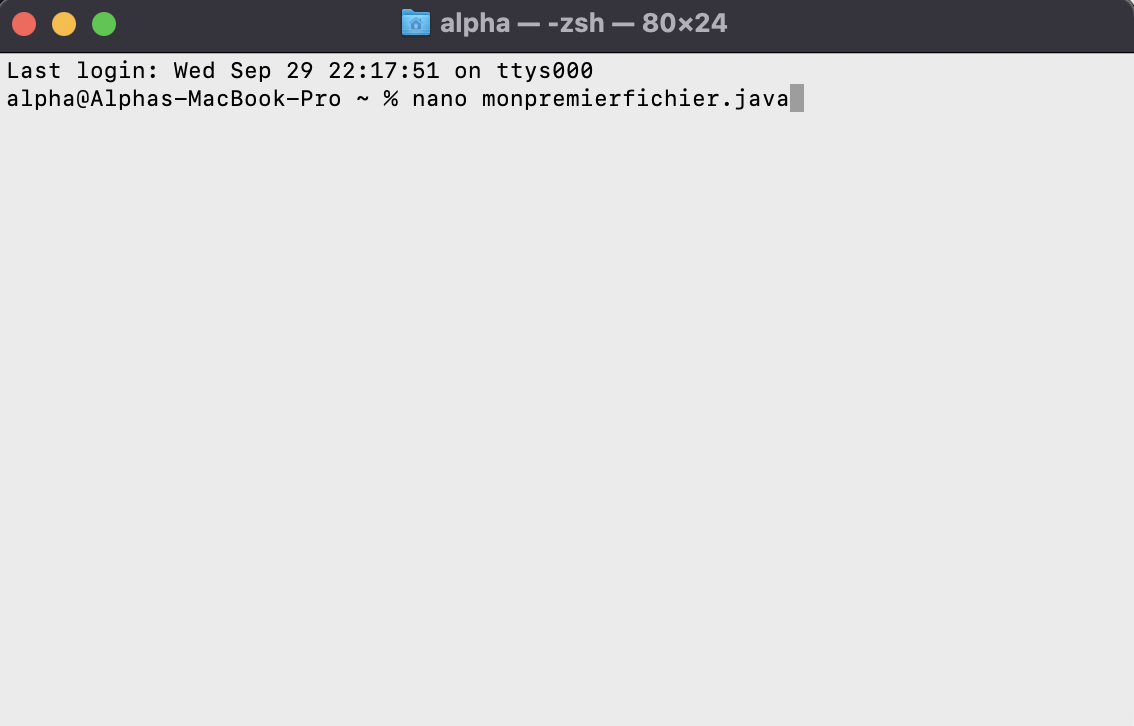
\includegraphics[width=12cm]{1_1j}	
\end{center}

\subsection{Création d'un programme en Java sur Windows}

Pour créer un fichier Python sur Windows, il suffit simplement d'entrer la commande \lstinline{notepad monpremierfichier.java} dans le bloc-note. Vous pouvez alors simplement l'éditer et l'enregistrer.

\begin{center}
	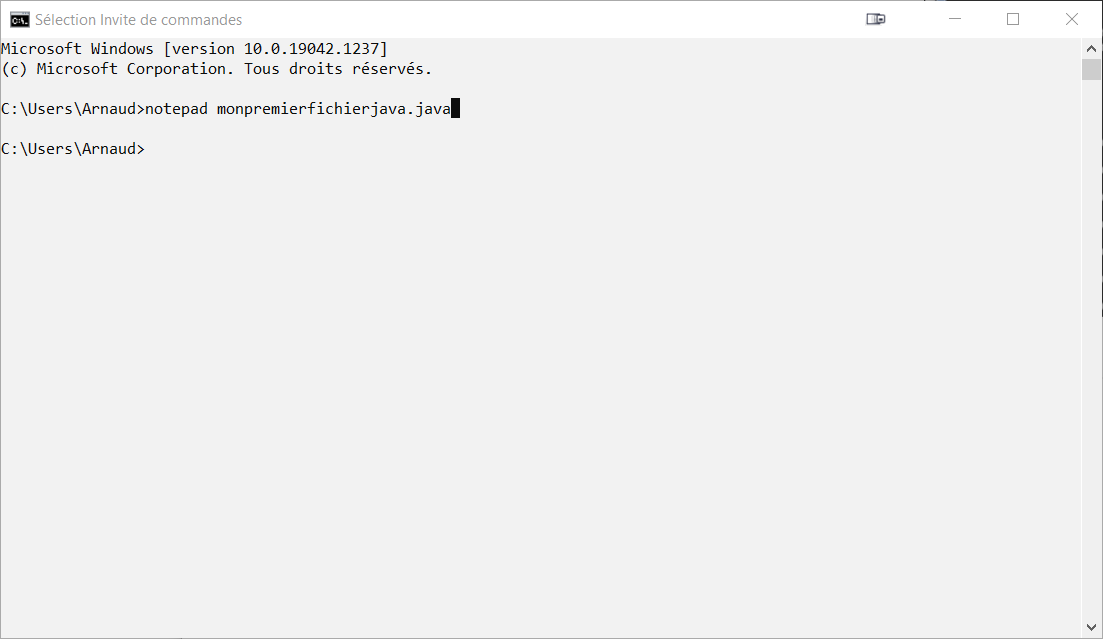
\includegraphics[width=12cm]{2j}
\end{center}
\begin{center}
	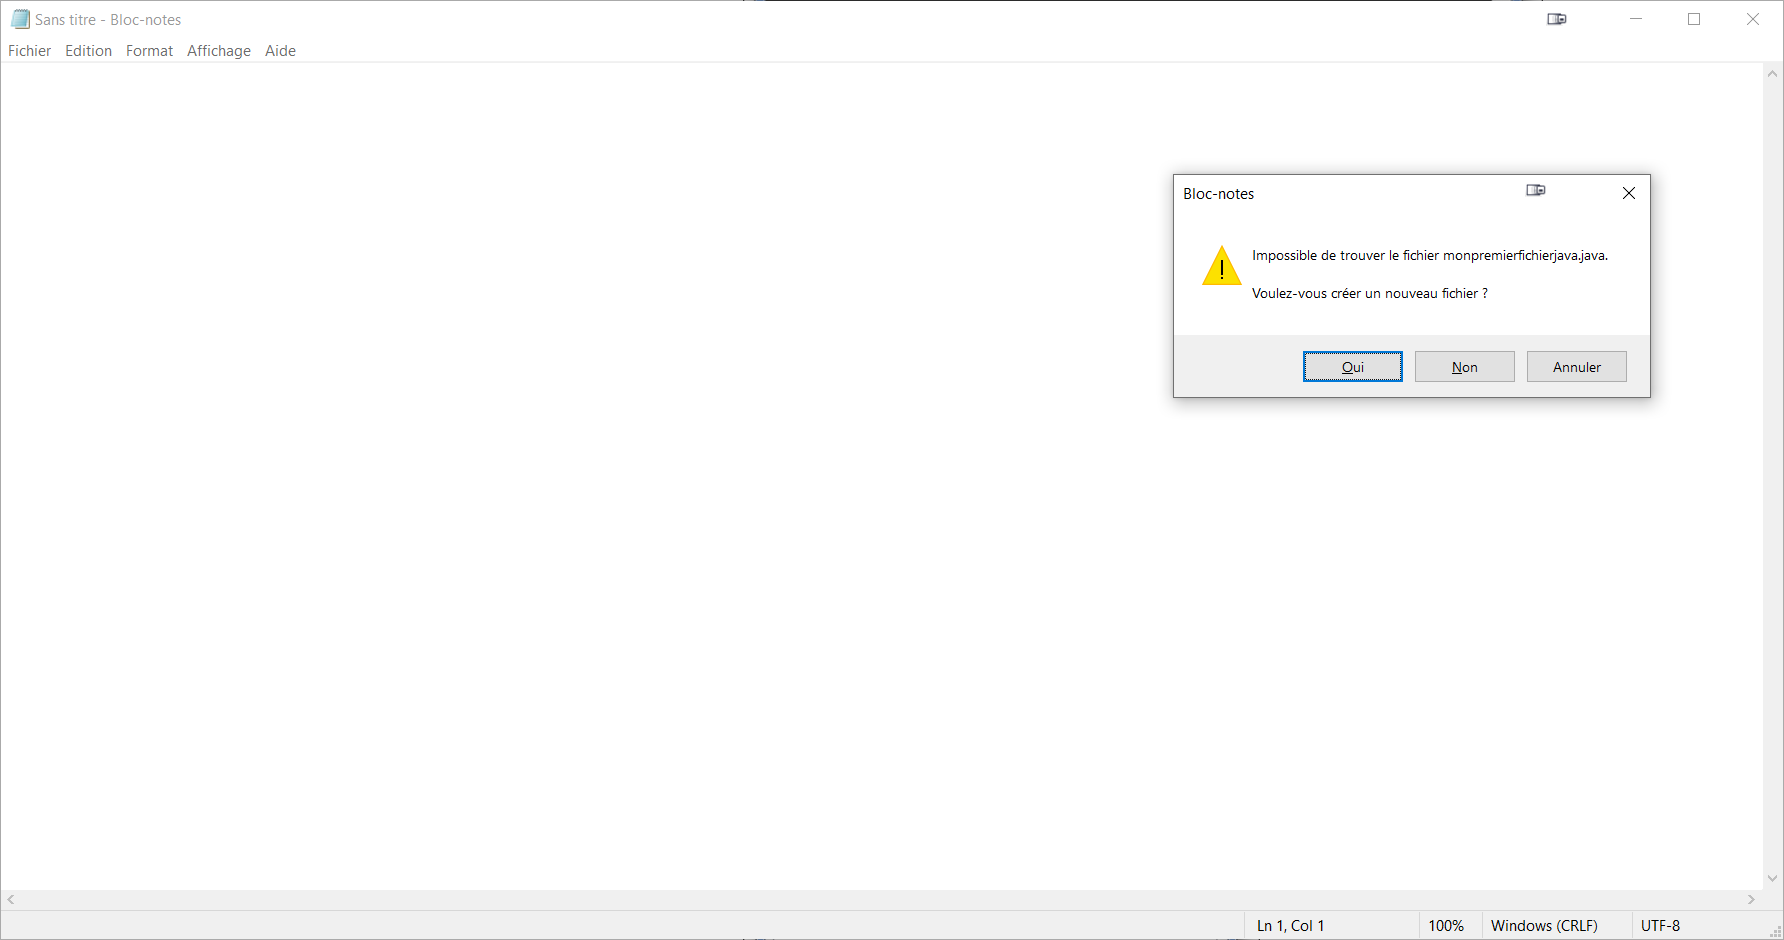
\includegraphics[width=12cm]{3j}
\end{center}

Pour éditer votre programme Java, il suffit simplement de l'éditer avec n'importe quel éditeur de texte.
Vous pouvez ensuite compiler et lancer votre programme Java en entrant les commandes \lstinline{javac monpremierfichierjava.java} et \lstinline{java monpremierfichierjava.java}. Ce dernier va s'exécuter dans le terminal.
\begin{center}
	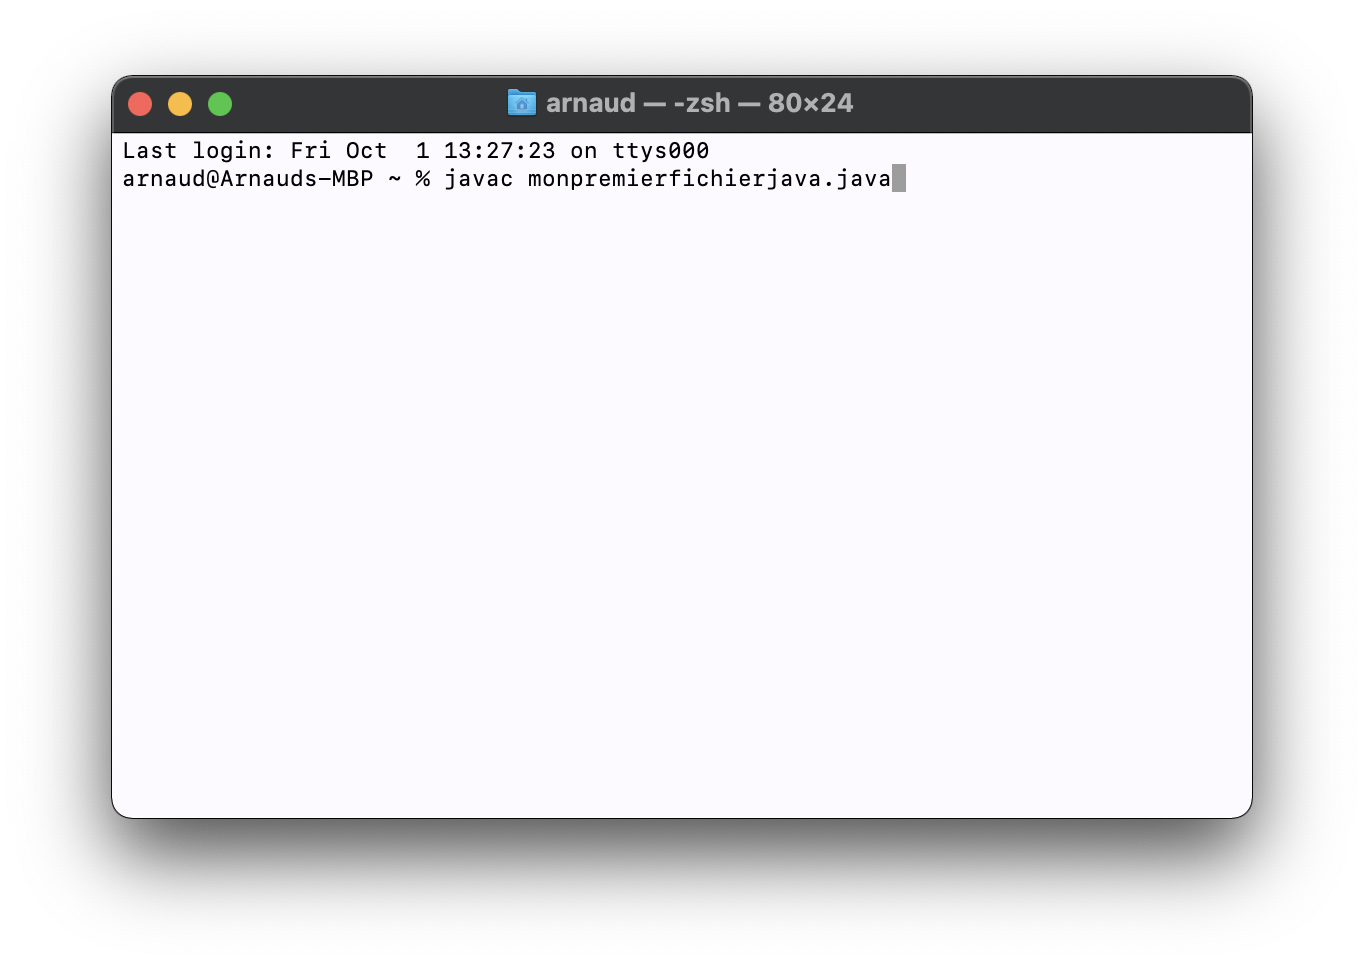
\includegraphics[width=12cm]{4j}
\end{center}
 

\subsection{IntelliJ IDEA}

Dans le cours, il vous a été demandé d'installer IntelliJ IDEA, l'un des environnements de développement le plus populaire de ces dernières années. Un environnement de développement ou IDE (Integrated Development Environnement) est un programme qui combine différents outils de développement et qui facilite le travail d'un programmeur. Pour ouvrir un fichier \lstinline{.java} avec le programme, il est nécessaire de créer un nouveau projet et de copier le fichier \lstinline{.java} dans le dossier contenant le projet.
\\\\
Commencez par ouvrir IDEA et créez un nouveau projet.

\begin{center}
	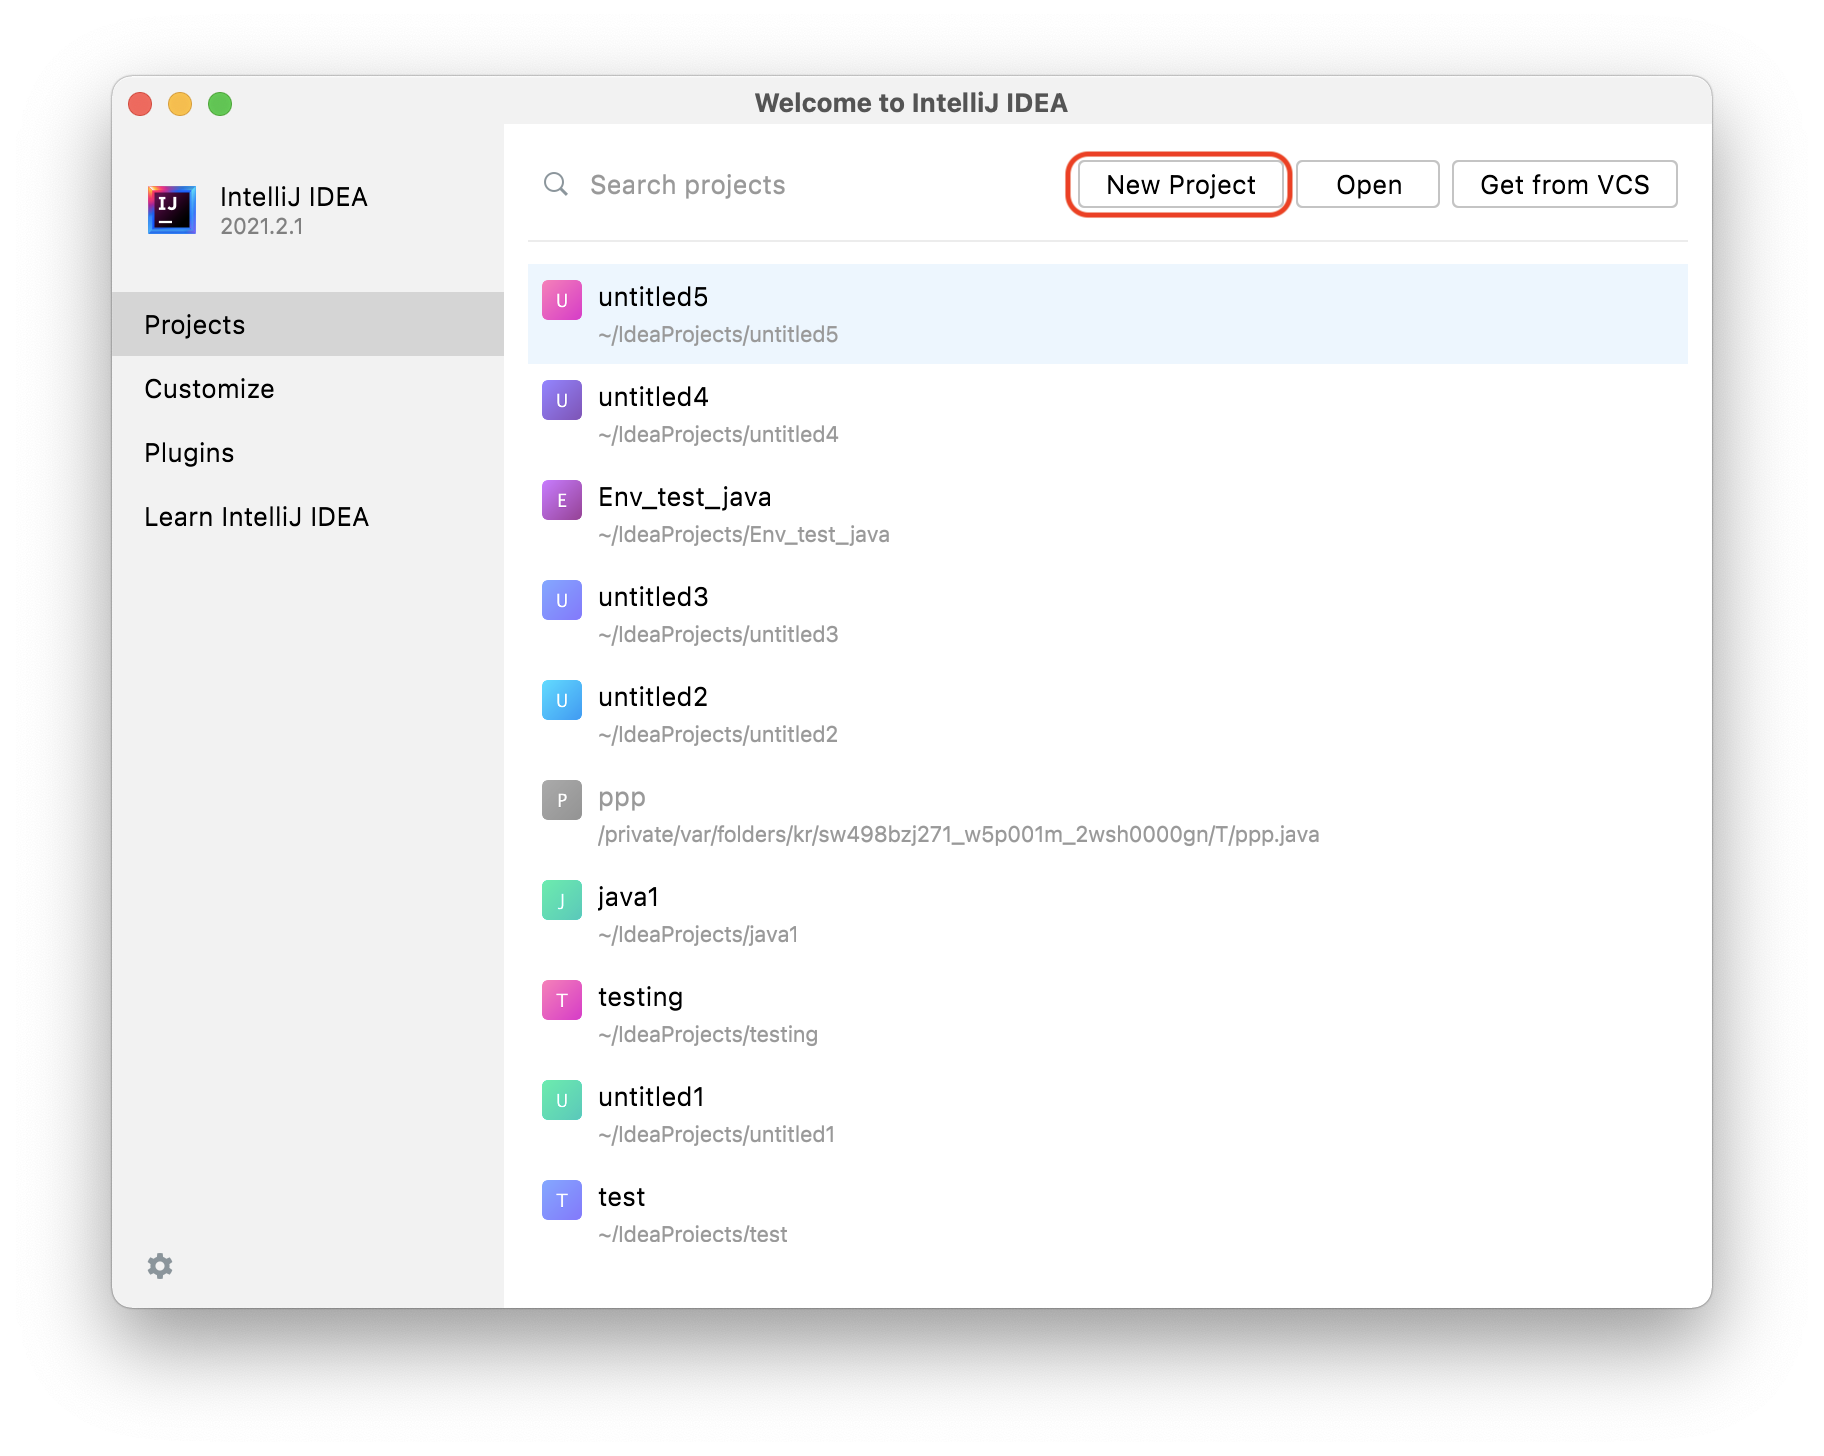
\includegraphics[width=12cm]{5j}	
\end{center}
 

Dans le menu à gauche, vous allez retrouver un sous-dossier nommé src. Ouvrez l'emplacement de ce dossier puis copiez le fichier .java que vous souhaitez lancer.

\begin{center}
	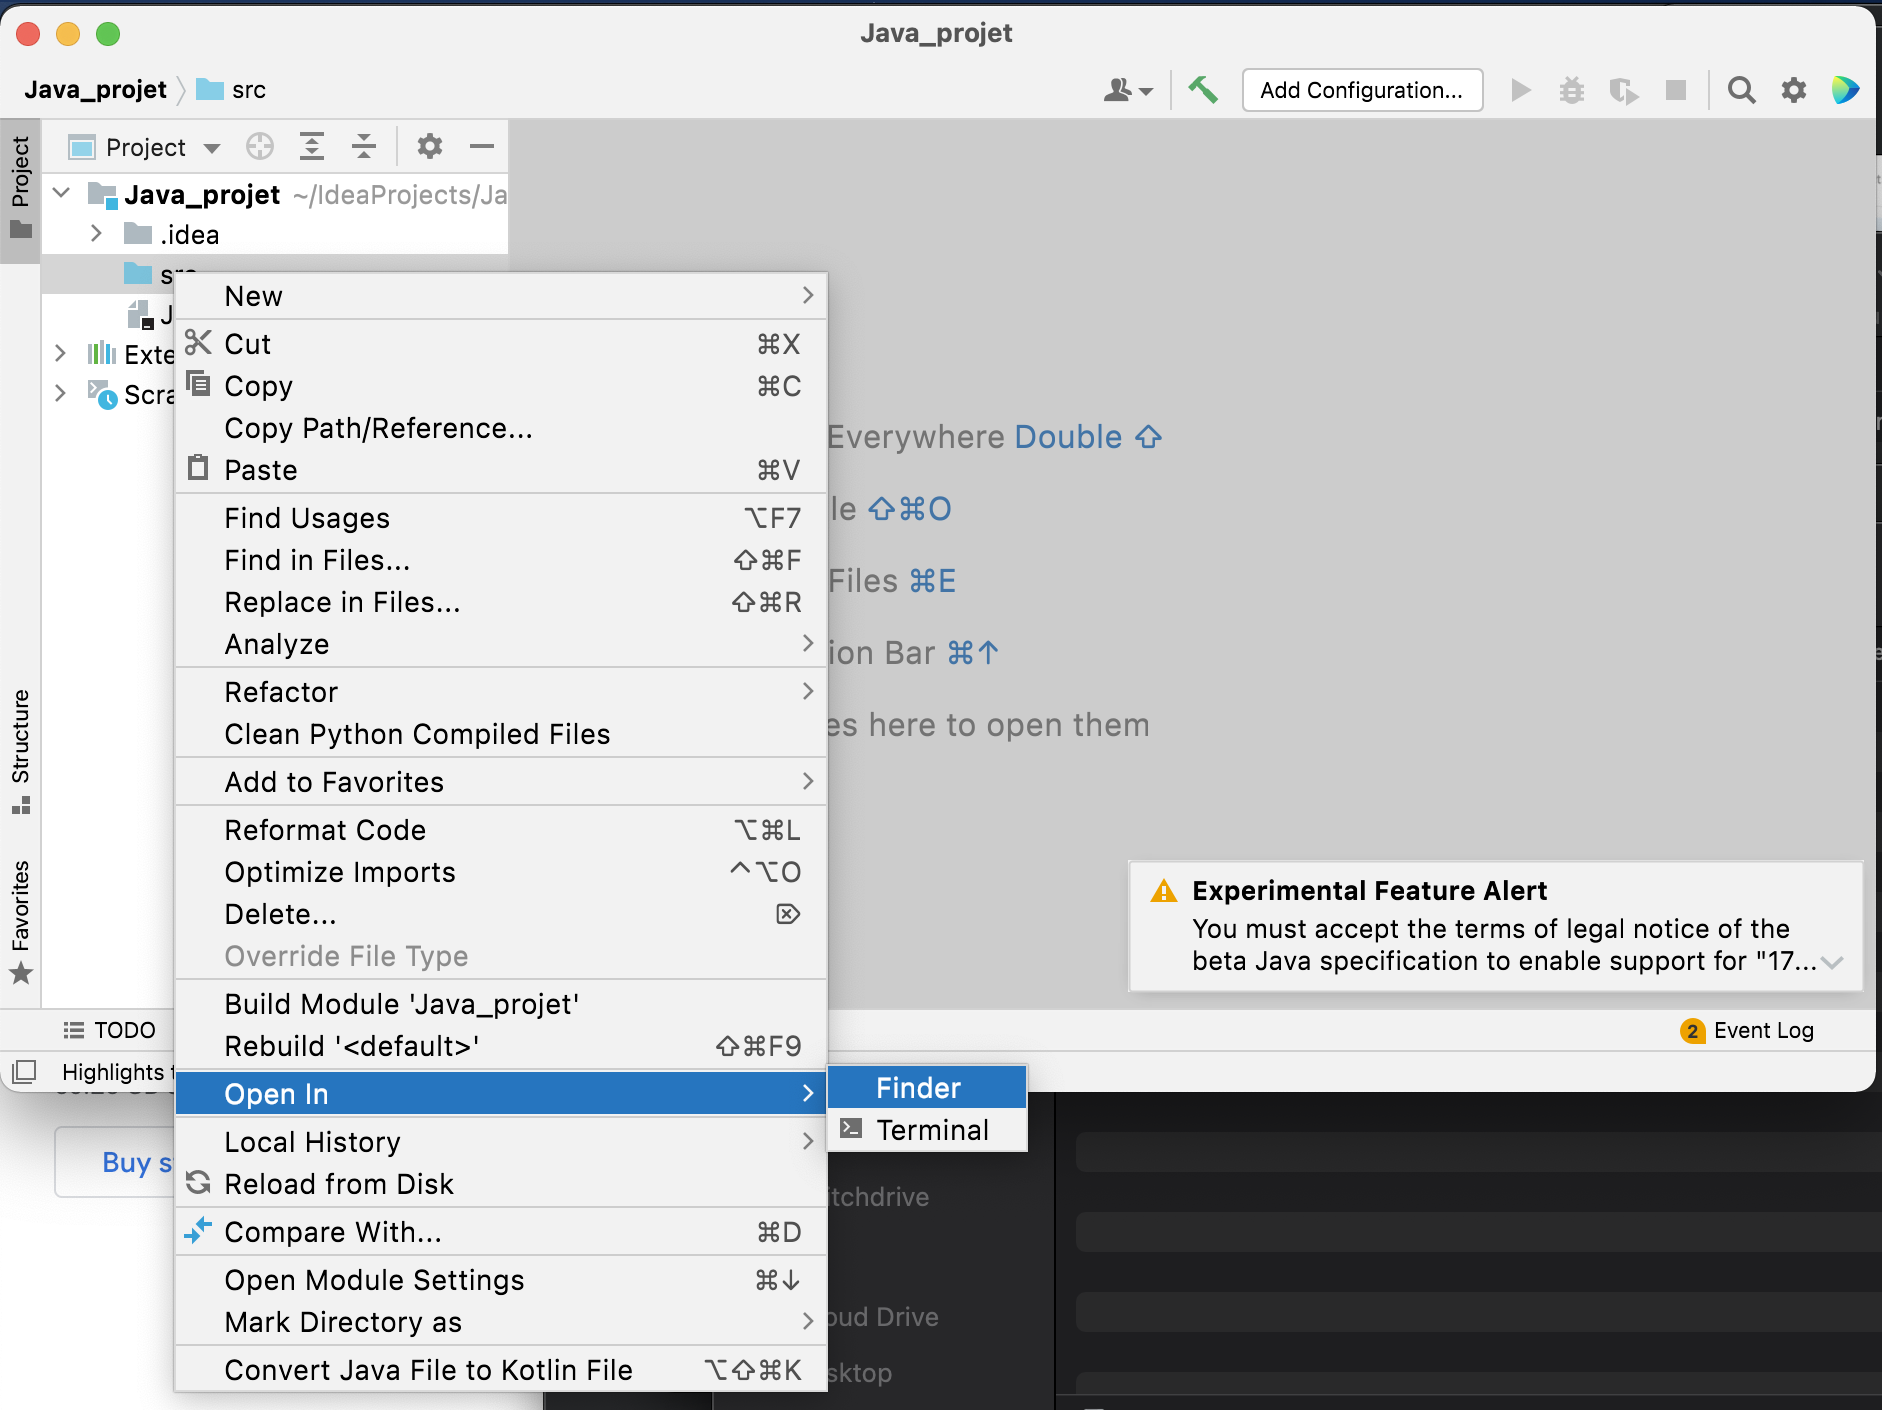
\includegraphics[width=12cm]{6j}	
\end{center}

La fenêtre qui vient de s'ouvrir est similaire à un éditeur de texte basique. C'est ici que le code peut être entré et modifié.

Vous pouvez maintenant lancer le fichier en allant dans \lstinline{Run... > Run lenomdevotreclasse}

\subsection{Les Classes en Java}

Contrairement à d'autres langages de programmation, tout code en Java doit être écrit à l'intérieur d'une classe. La notion de classe vous sera présentée plus en détails dans la suite du cours.

\begin{comment}
Une classe en Java est semblable à une sorte de schéma pour créer ce qu'on appelle des objets. Les objets sont donc des instances particulières d'une certaine classe. Par exemple, ``l'objet'' Basketball serait une instance de la ``classe'' Sport. Pour créer une classe en Java, il suffit d'écrire \lstinline{class Lenomdemaclasse}
\end{comment}

\begin{center}
	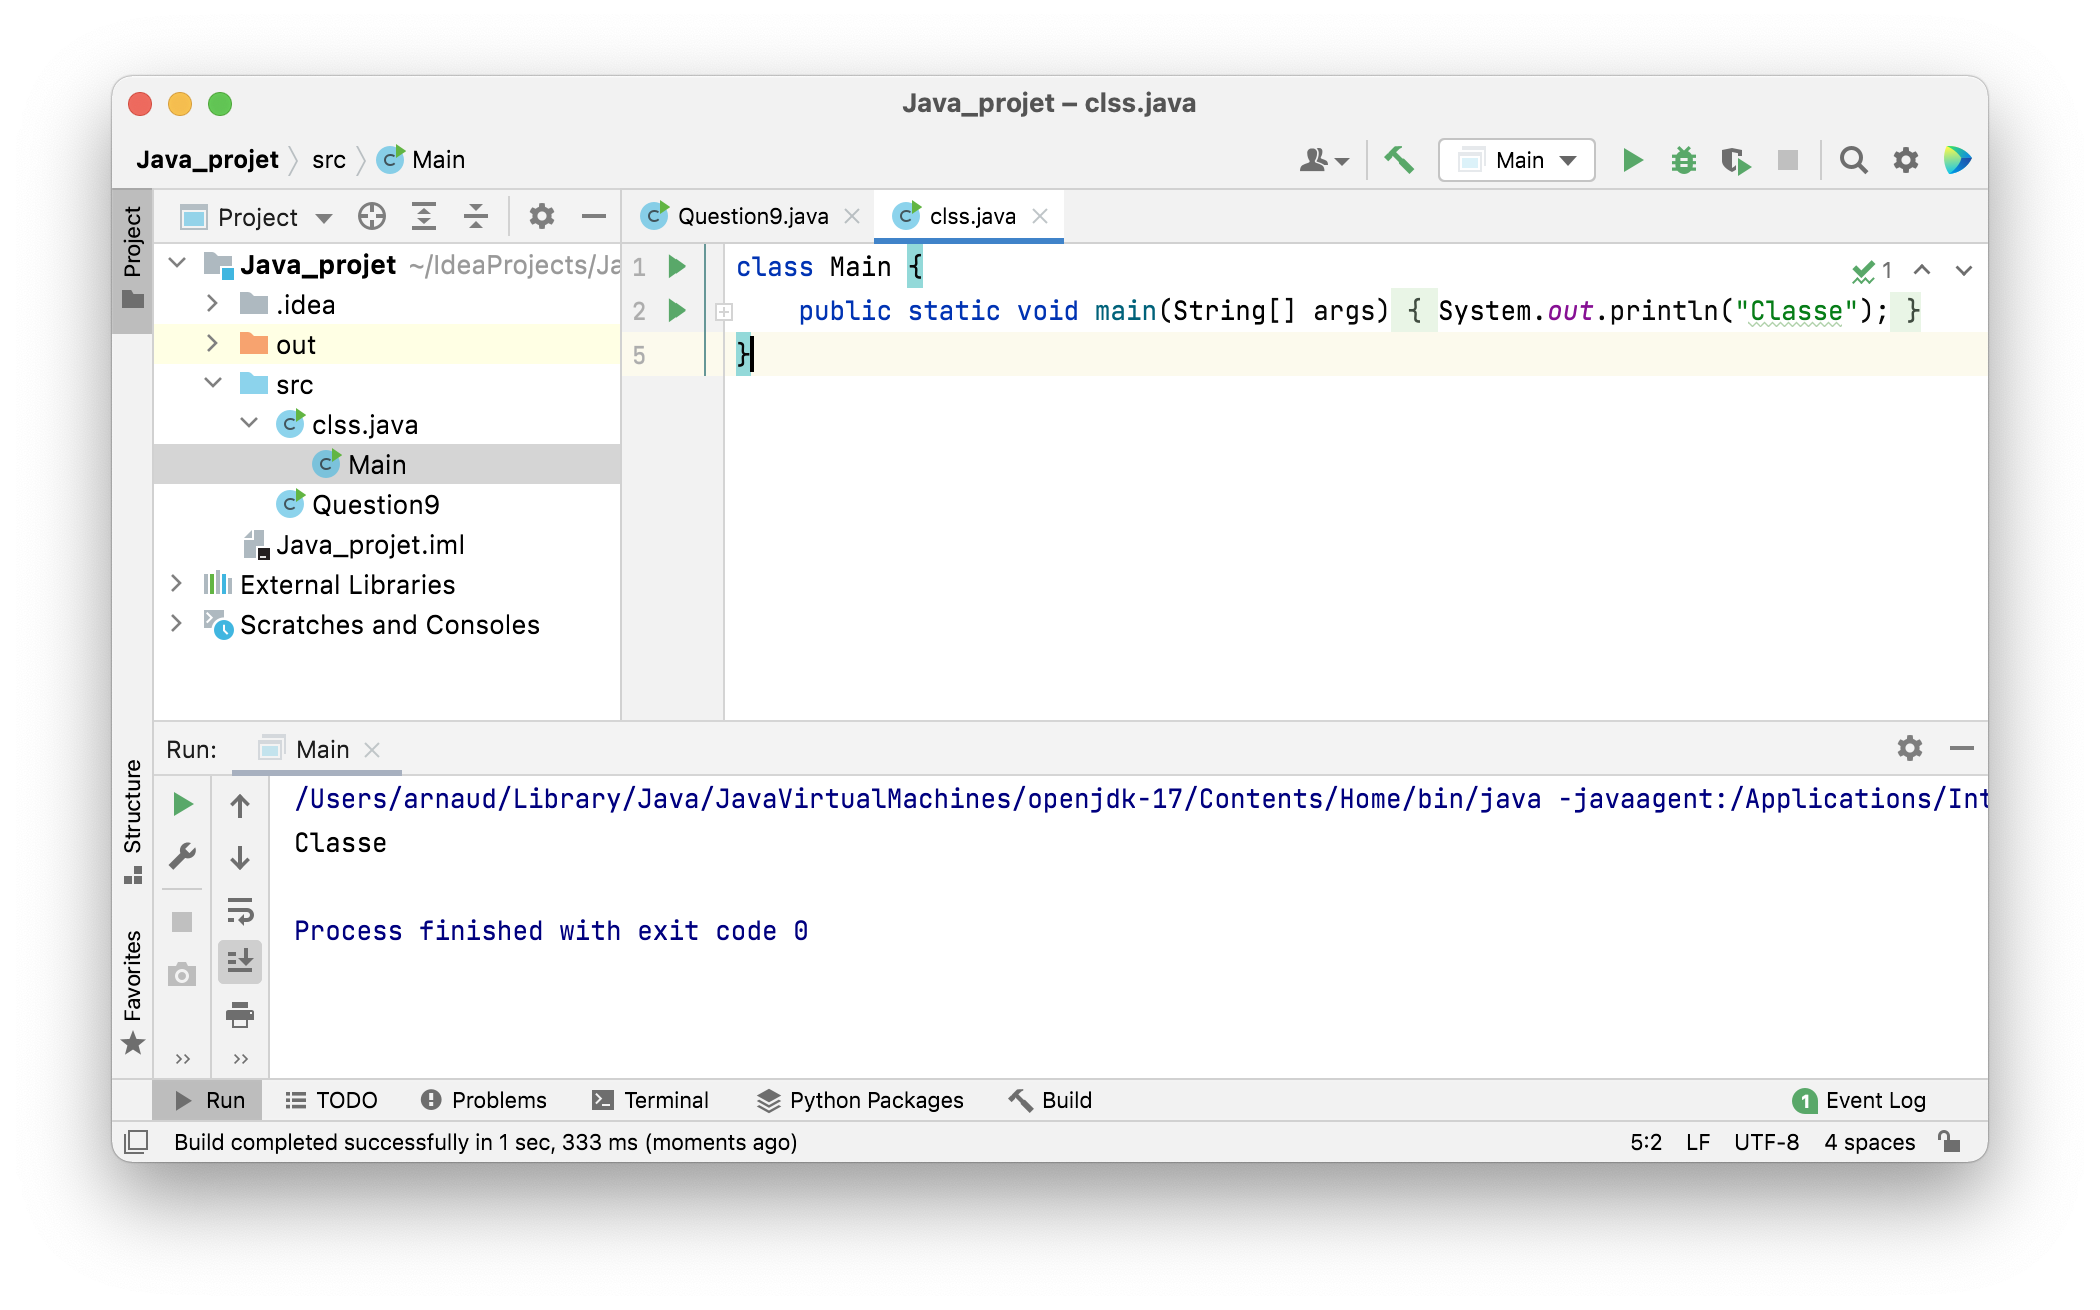
\includegraphics[width=12cm]{7j}	
\end{center}

\subsection{La méthode main}
Dans tout programme Java, on doit toujours retrouver au moins une fois la fonction \lstinline{public static void main(String[] args)} dans une de nos classes. Cette fonction est un point d'entrée dans le programme qui ne s'exécutera pas s'il ne retrouve pas cette fonction.

\subsection{La création de variables}

Les variables dans les langages de programmation sont similaires à des noms données à une valeur précise.
Pour assigner une valeur à une variable en Java, il suffit de respecter le format suivant \lstinline{type variable=valeur}.


\begin{conseil}
\begin{itemize}
	\item On peut assigner n'importe quelle suite de caractères non-réservée en tant que variable
	\item Il est aussi possible d'assigner des chaînes de caractères (strings en anglais) ou encore des valeurs booléennes à des variables
	\item En réassignant une nouvelle valeur à une variable déjà définie, la valeur de la variable va être écrasée et remplacée par la nouvelle valeur
	\item Il est possible d'additionner les variables du même type
	\item Plusieurs variables peuvent avoir la même valeur
	\item Le nom d'une variable doit toujours commencer par une lettre
\end{itemize}

\end{conseil}
À noter que les dernières versions de Java supportent l'inférence du type des variables. On pourrait autant écrire \lstinline{String a="abc"} que \lstinline{a="abc"} car le type de la variable serait automatiquement défini. 
Dans le cadre du cours, nous vous recommandons de toujours déclarer le type de vos variables.

Si vous ouvrez et exécutez le programme Java \lstinline{Variables.java} qui contient quelques exemples d'attribution de variables, vous pourrez observer comment sont créées différentes variables mais aussi comment le programme les traite.
\begin{center}
	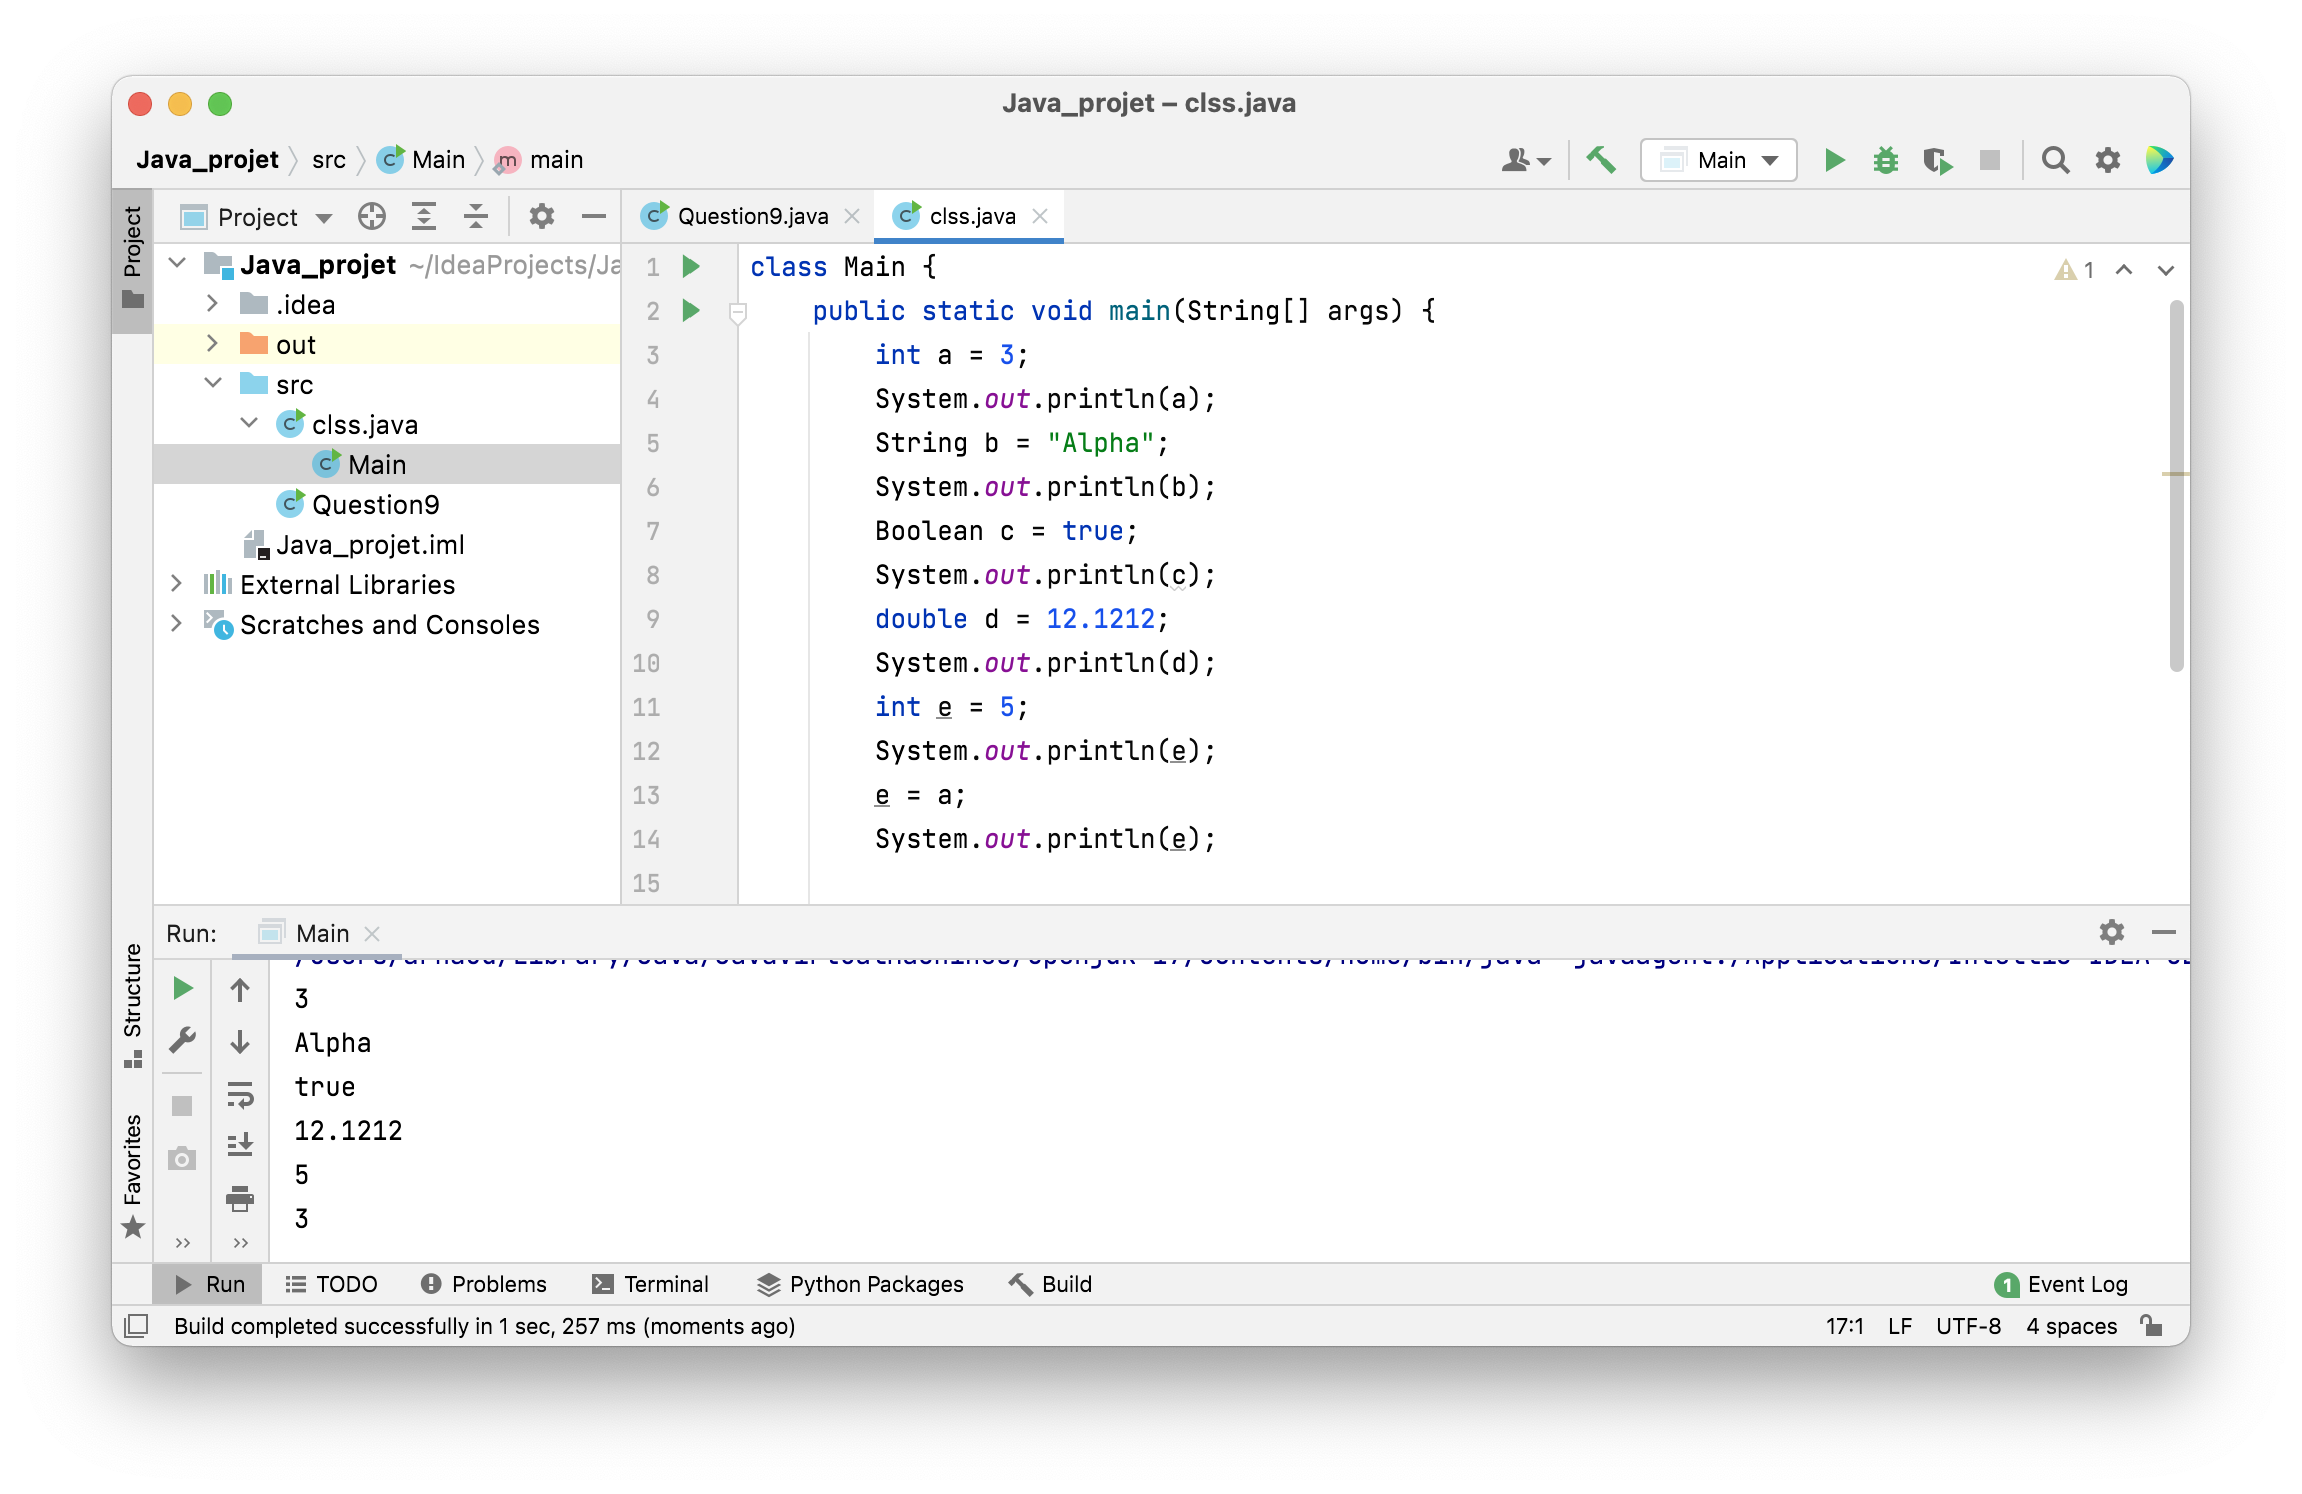
\includegraphics[width=12cm]{8j}	
\end{center}

\subsection{Les fonctions}

Dans les langages de programmation, on retrouve un très grand nombre de fonctions. Ces fonctions sont des blocs de code qui, lorsqu'ils sont invoqués avec certains paramètres, effectuent certaines actions. Une des fonctions basique et plutôt importante en Java est la fonction \lstinline{System.out.println("Votremessage");}.  Cette dernière permet d'afficher à l'écran le contenu de la parenthèse.\\ 
Si vous entrez la ligne de code \lstinline{System.out.println("Votremessage");} et que vous lancez le programme, IntelliJ va vous afficher une ligne de texte. Le message qui apparaît est celui que vous avez entré entre guillemets (à la place de ''Votremessage``'). C'est le but d'une fonction \lstinline{System.out.println("Votremessage");}
\begin{center}
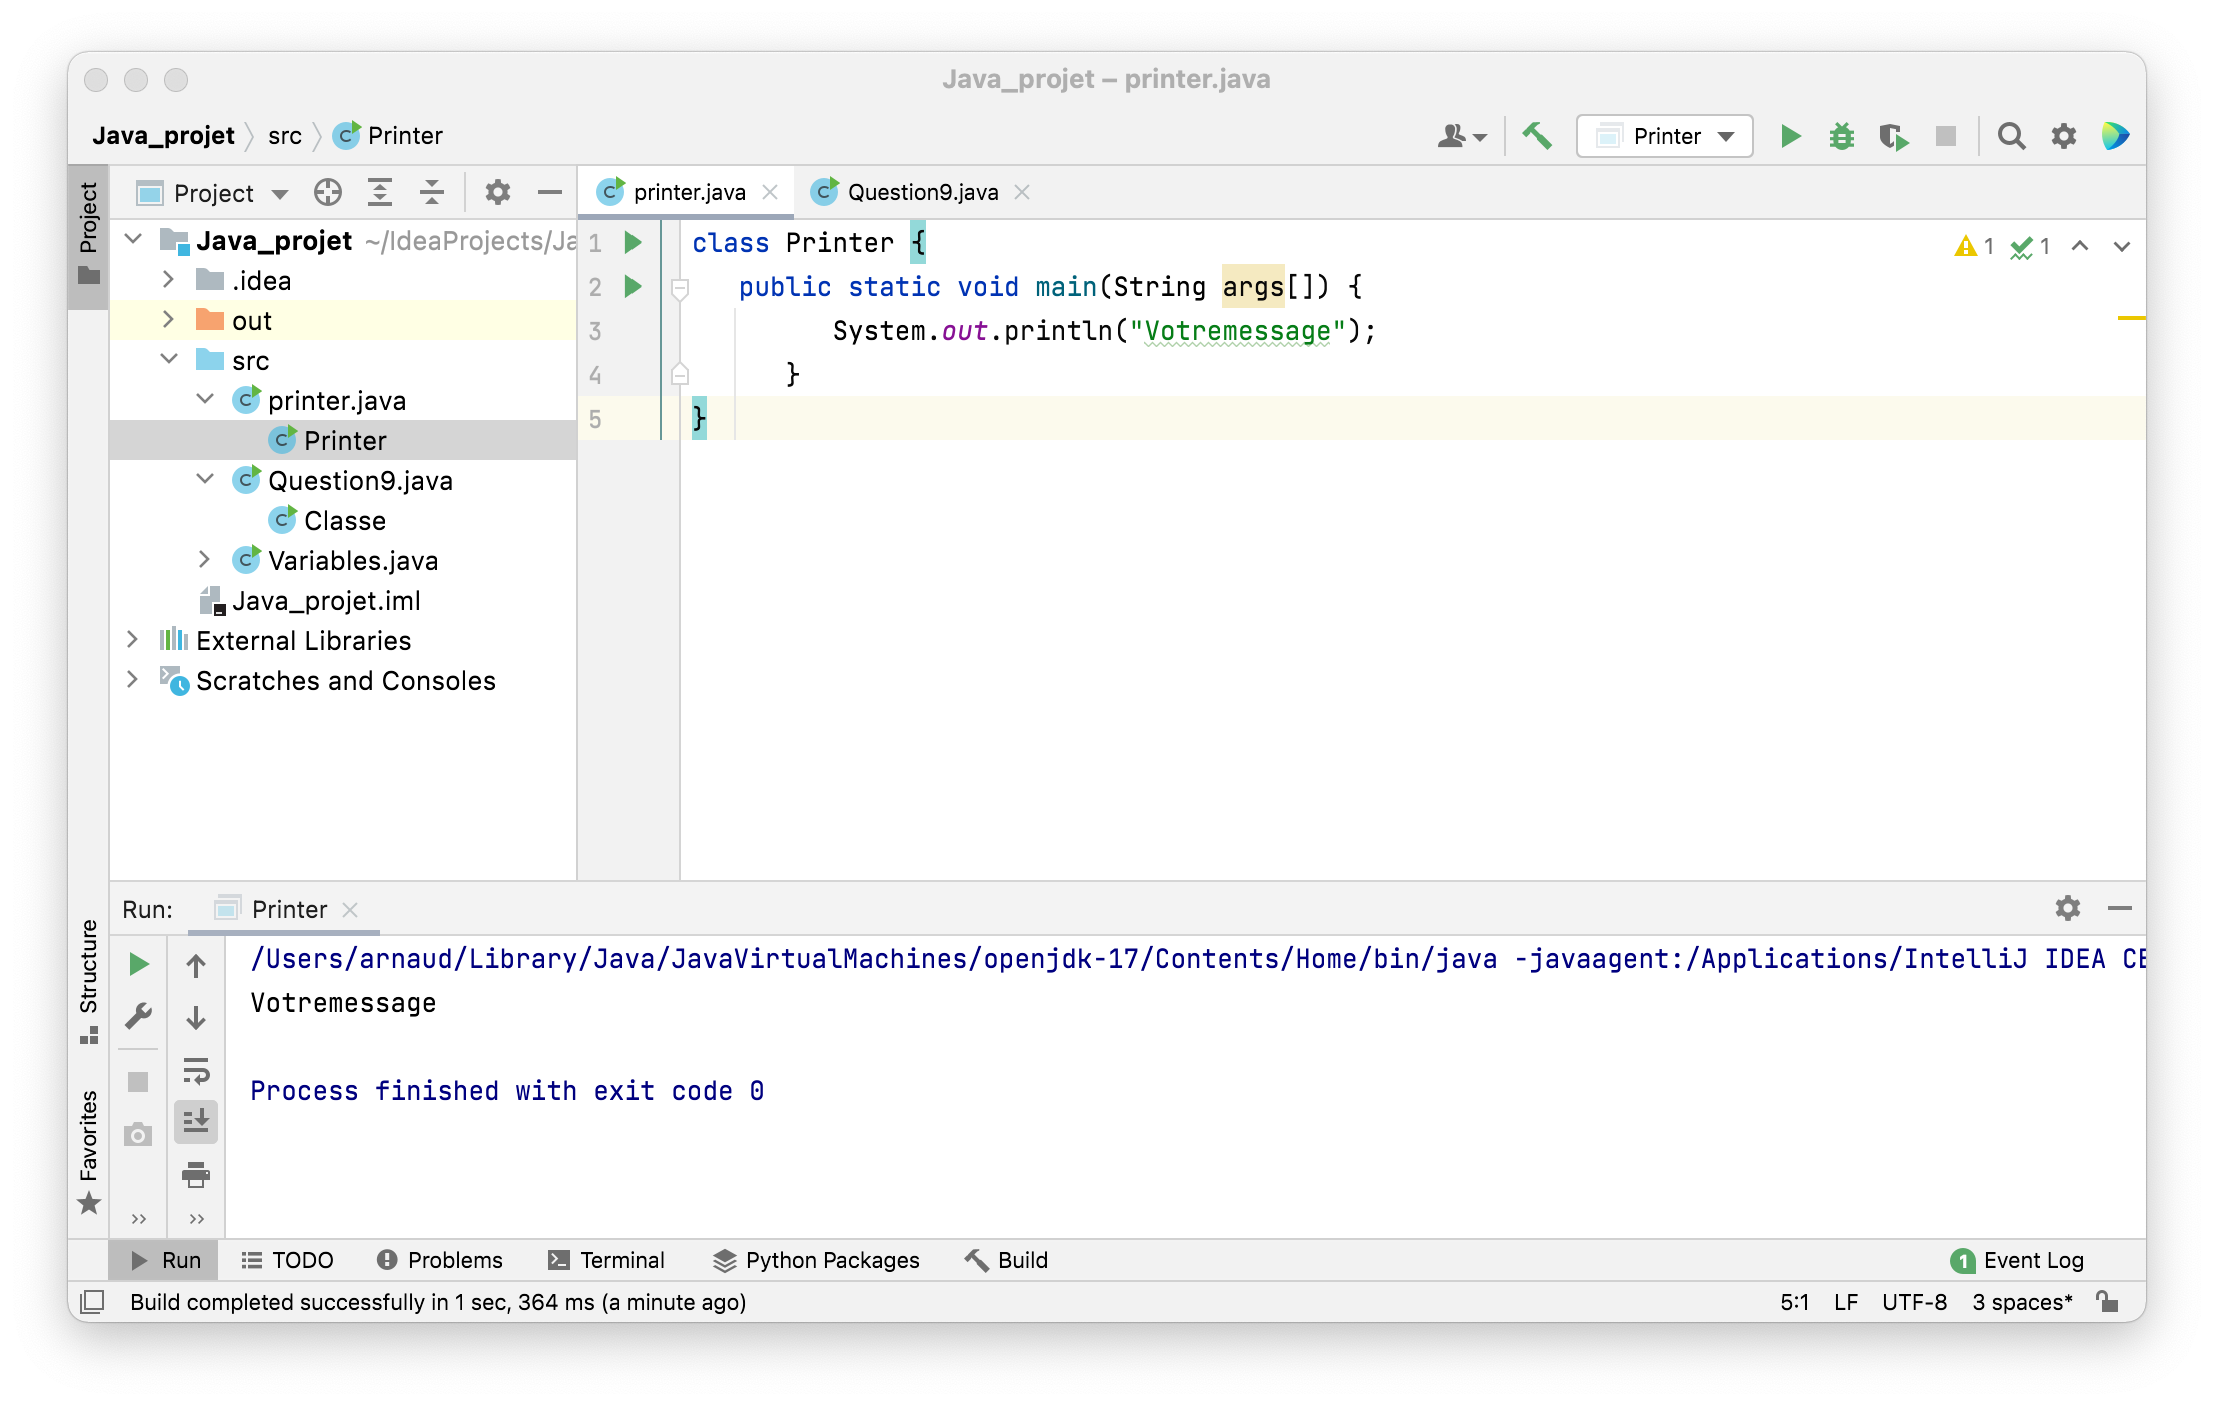
\includegraphics[width=12cm]{9j}	
\end{center}


En plus des fonctions incluses dans les librairies de base, il est possible de créer des fonctions complètement personnalisées (généralement plusieurs fonctions sont réunies en une seule) au moyen de la fonction \lstinline{static void nomdelafonction() } et de l'utiliser à n'importe quel moment en l'invoquant avec \lstinline{nomdelafonction()}.

Si vous ouvrez et exécutez le programme \lstinline{mafonction.java}, vous pourrez voir l'exemple de la fonction personnalisée \lstinline{mafonction} qui imprime 3 suites de caractères différentes.

\begin{center}
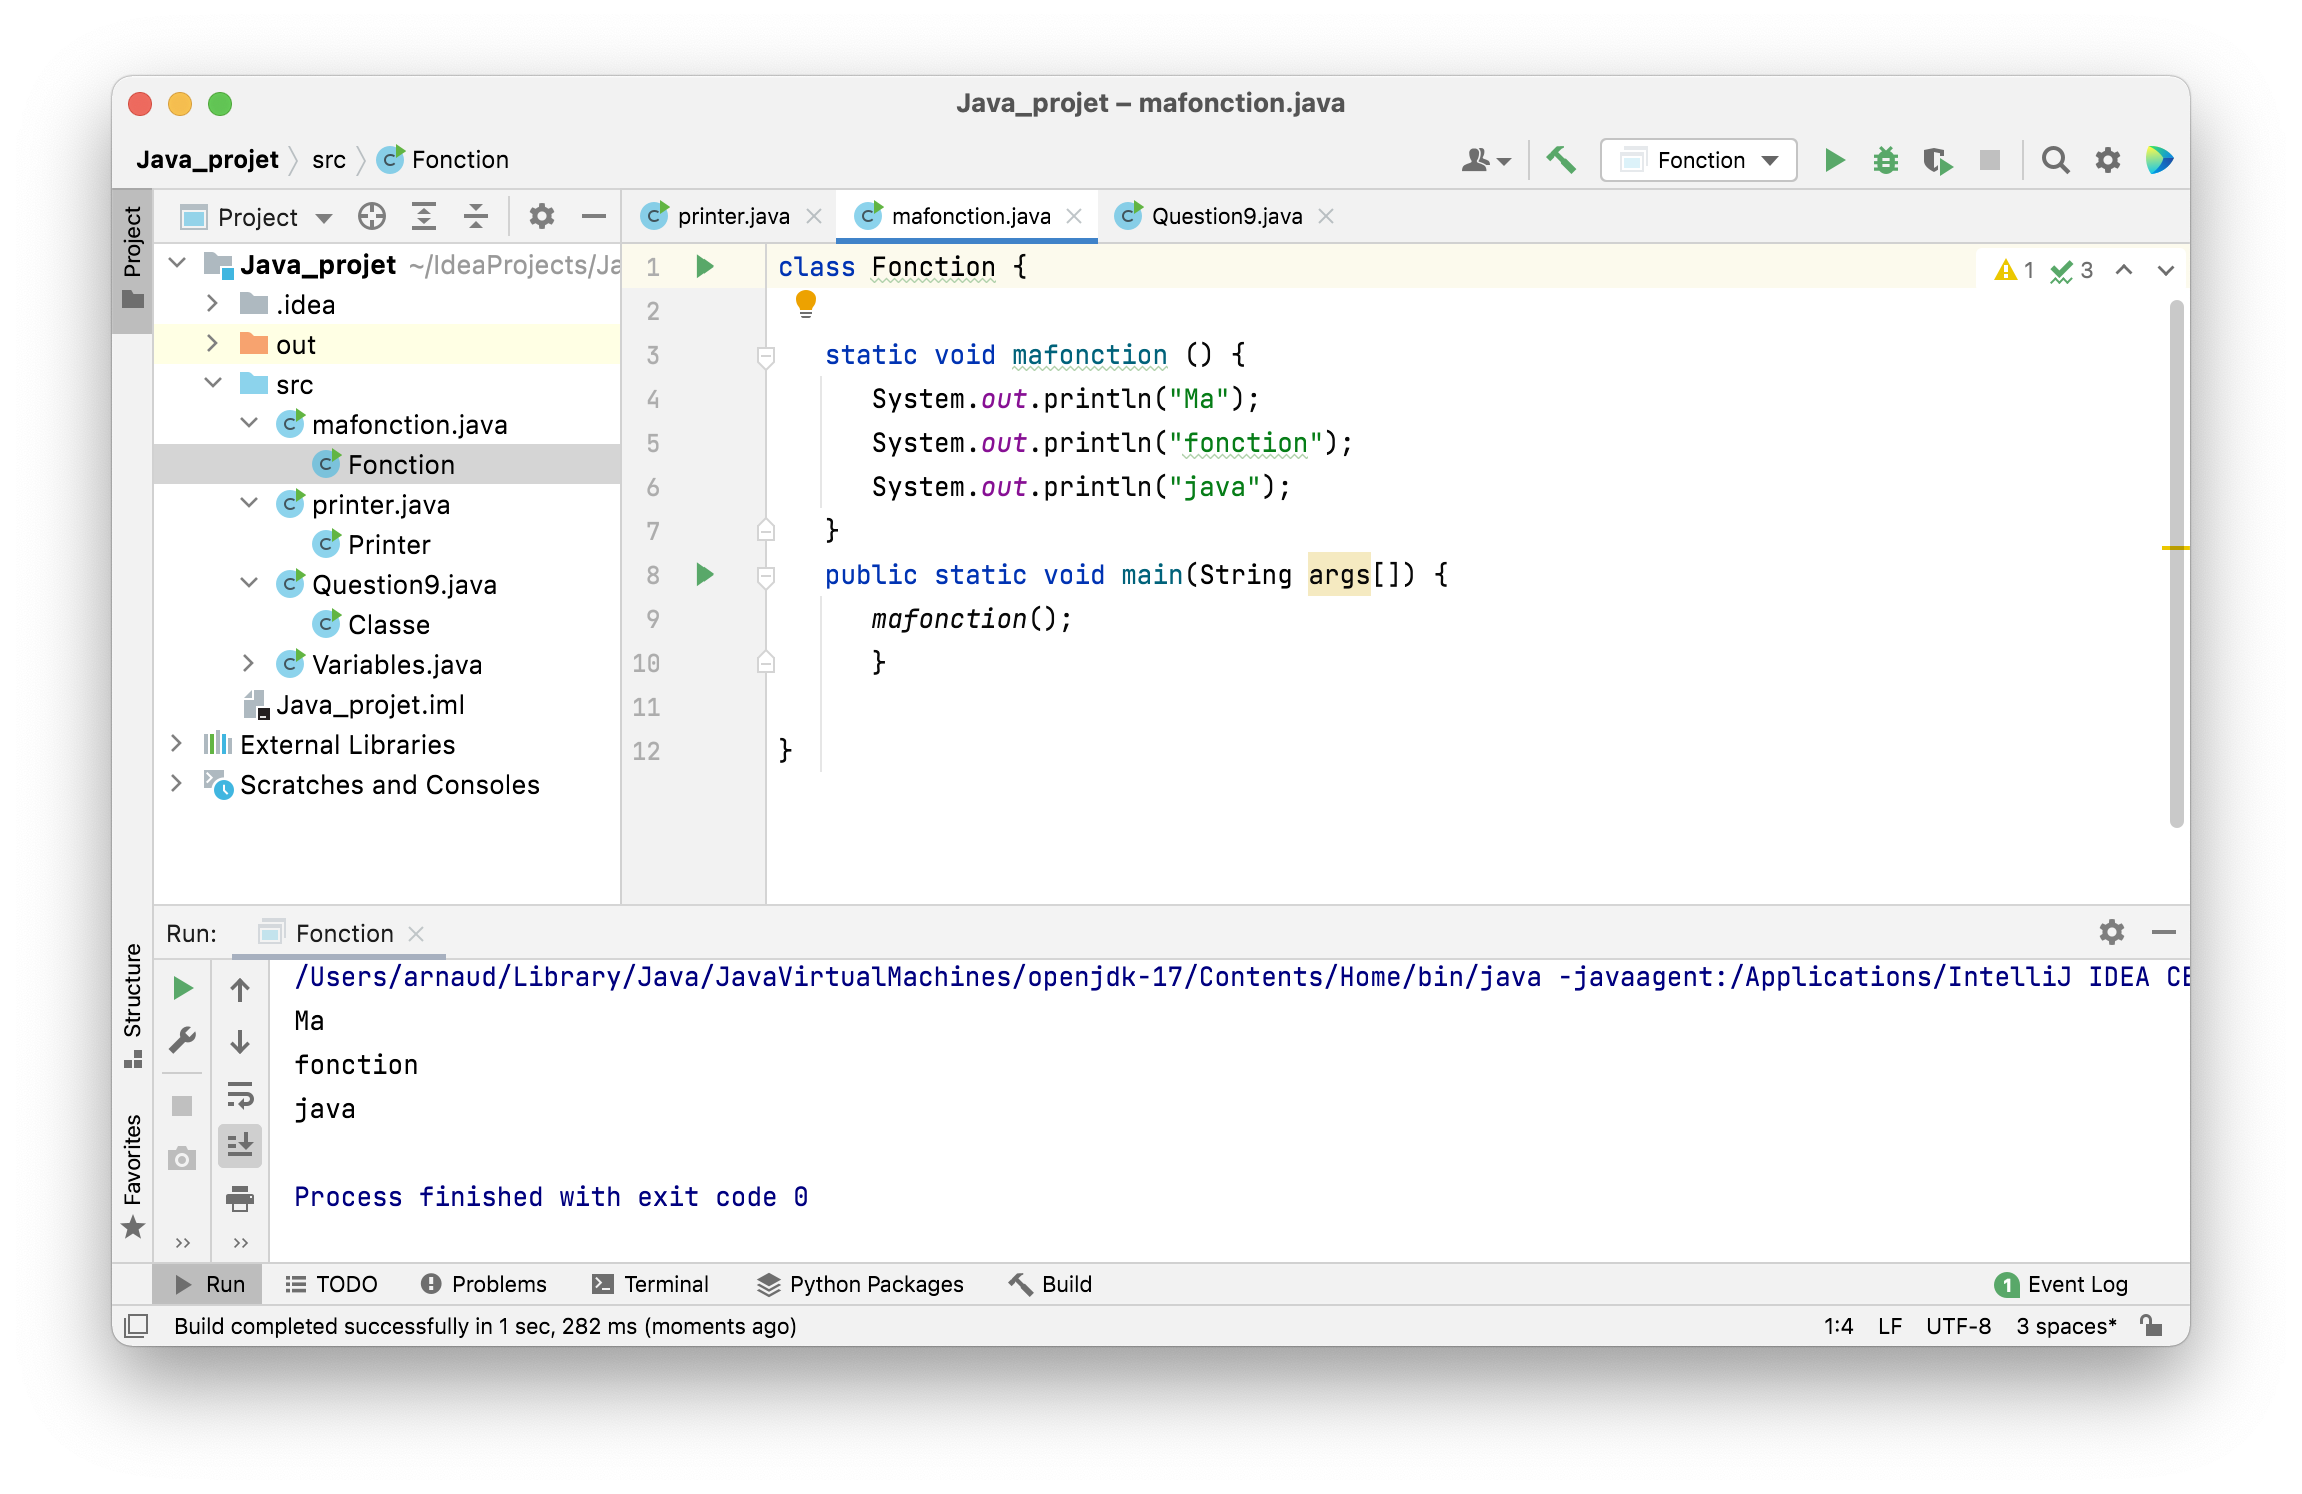
\includegraphics[width=12cm]{10j}		
\end{center}

\end{document}
